\chapter{Foundation for inference}
\label{foundationsForInference}

In the last chapter we encountered a probability problem in which we calculated the chance of getting less than 15\% smokers in a sample, if we \emph{knew} the true proportion of smokers in the population was 0.20. This chapter introduces the topic of inference, that~is, the methods of drawing conclusions when the population value is \emph{unknown}.

\begin{termBox}{\tBoxTitle{Probability versus inference}
\vspace{-5mm}
\begin{description}
\item[Probability] Probability involves using a known population value (parameter) to make a prediction about the likelihood of a particular sample value (statistic).
\item[Inference] Inference involves using a calculated sample value (statistic) to estimate or better understand an unknown population value (parameter).
\end{description}
}
\end{termBox}

Statistical inference is concerned primarily with understanding the quality of parameter estimates. In this chapter, we will focus on the case of estimating a proportion from a random sample. While the equations and details change depending on the setting, the foundations for inference are the same throughout all of statistics. We introduce these common themes in this chapter, setting the stage for inference on other parameters. Understanding this chapter will make the rest of this book, and indeed the rest of statistics, seem much more familiar.



\textA{\newpage}

\section[Estimating unknown parameters]{Estimating unknown parameters \sectionvideohref{youtube-DNIauUrRIEM&list=PLkIselvEzpM7Pjo94m1e7J5jkIZkbQAl4} \sectionslideshref{gdoc_aps_slides_5-1}}
\subsection{Point estimates}
\label{pointEstimates}

\index{point estimate!single proportion|(}

\begin{example}{We take a sample of size $n=80$ from a particular county and find that 12 of the 80 people smoke. Estimate the \term{population proportion} based on the sample. Note that this example differs from Example~\ref{smokers} of the previous chapter in that we are not trying to predict what will happen in a sample. Instead, we have a sample, and we are trying to infer something about the true proportion.} The most intuitive way to go about doing this is to simply take the \term{sample proportion}. That is,
$\hat{p} = \frac{12}{80} = 0.15$ is our best estimate for $p$, the population proportion.
\end{example}

The sample proportion $\hat{p} = 0.15$ is called a \term{point estimate} of the population proportion: if we can only choose one value to estimate the population proportion, this is our best guess. Suppose we take a new sample of 80 people and recompute the proportion of smokers in the sample; we will probably not get the exact same answer that we got the first time. Estimates generally vary from one sample to another, and this \term{sampling variation} tells us how close we expect our estimate to be to the true parameter.

\begin{example}{
In Chapter~\ref{summarizingData}, we found the summary statistics for the number of characters in a set of 50 email data. These values are summarized below.

\begin{tabular}{l r }
$\bar{x}$ & 11,160 \\
median & 6,890 \\
$s_x$ & 13,130
\end{tabular}

Estimate the \term{population mean} based on the sample.}The best estimate for the population mean is the \term{sample mean}. That is,
$\bar{x} = 11,160$ is our best estimate for $\mu$.
\end{example}

\begin{exercise}Using the email data, what quantity should we use as a point estimate for the population standard deviation $\sigma$?\footnote{Again, intuitively we would use the sample standard deviation $s = 13,130$ as our best estimate for $\sigma$.}
\end{exercise}

%\Comment{add this discussion along with graphs for second edition?}
%\Cut{
%We will say that point estimate is \term{accurate} if the average of all of its possible values is the true population parameter. We will say that a point estimate is \term{precise} if it has low variability.
%
%Why do we want a point estimate to be both accurate and precise?
%}

\subsection{Introducing the standard error}

Point estimates only approximate the population parameter, and they vary from one sample to another. It will be useful to quantify how variable an estimate is from one sample to another. For a random sample, when this variability is small we can have greater confidence that our estimate is close to the true value.

How can we quantify the expected variability in a point estimate $\hat{p}$? The discussion in Section~\ref{distributionphat} tells us how. The variability in the distribution of $\hat{p}$ is given by its standard deviation.
\begin{align*}
SD_{\hat{p}}&=\sqrt{\frac{p(1-p)}{n}}
\end{align*}

\textA{\pagebreak}

\begin{example}{Calculate the standard deviation of $\hat{p}$ for smoking example, where $\hat{p}$ = 0.15 is the proportion in a sample of size 80 that smoke.}It may seem easy to calculate the $SD$ at first glance, but there is a serious problem: $p$ is \emph{unknown}. In fact, when doing inference, $p$ must be unknown, otherwise it is illogical to try to estimate it. We cannot calculate the $SD$, but we can estimate it using, you might have guessed, the sample proportion $\hat{p}$.
\end{example}
 
This estimate of the standard deviation is known as the \termsub{standard error}{standard error ($SE$)}, or \term{$SE$} for short.
\begin{align*}
SE_{\hat{p}}&=\sqrt{\frac{\hat{p}(1-\hat{p})}{n}}
\end{align*}

\begin{example}{Calculate and interpret the $SE$ of $\hat{p}$ for the previous example.}
\begin{align*}
SE_{\hat{p}}=\sqrt{\frac{\hat{p}(1-\hat{p})}{n}} =\sqrt{\frac{0.15(1-0.15)}{80}}=0.04
\end{align*}
The average or expected error in our estimate is 4\%.
\end{example}

\begin{example}{If we quadruple the sample size from 80 to 320, what will happen to the $SE$?}
\begin{align*}
SE_{\hat{p}}=\sqrt{\frac{\hat{p}(1-\hat{p})}{n}} =\sqrt{\frac{0.15(1-0.15)}{320}}=0.02
\end{align*}
The larger the sample size, the smaller our standard error. This is consistent with intuition: the more data we have, the more reliable an estimate will tend to be. However, quadrupling the sample size does not reduce the error by a factor of 4. Because of the square root, the effect is to reduce the error by a factor $\sqrt{4}$, or 2. 
\end{example}


\subsection{Basic properties of point estimates}

We achieved three goals in this section. First, we determined that point estimates from a sample may be used to estimate population parameters. We also determined that these point estimates are not exact: they vary from one sample to another. Lastly, we quantified the uncertainty of the sample proportion using what we call the standard error. We will learn how to calculate the standard error for other point estimates such as a mean, a difference in means, or a difference in proportions in the chapters that follow. 

%_________________
\section[Confidence intervals]{Confidence intervals \sectionvideohref{youtube-FUaXoKdCre4&list=PLkIselvEzpM7Pjo94m1e7J5jkIZkbQAl4} \sectionslideshref{gdoc_aps_slides_5-2}}
\label{ConfidenceIntervals}

\index{confidence interval|(}

A point estimate provides a single plausible value for a parameter. However, a point estimate is rarely perfect; usually there is some error in the estimate. In addition to supplying a point estimate of a parameter, a next logical step would be to provide a plausible \emph{range of values} for the parameter.


\subsection{Capturing the population parameter}

A plausible range of values for the population parameter is called a \term{confidence interval}. Using only a point estimate is like fishing in a murky lake with a spear, and using a confidence interval is like fishing with a net. We can throw a spear where we saw a fish, but we will probably miss. On the other hand, if we toss a net in that area, we have a good chance of catching the fish.

If we report a point estimate, we probably will not hit the exact population parameter. On the other hand, if we report a range of plausible values -- a confidence interval -- we have a good shot at capturing the parameter.

\begin{exercise}
If we want to be very confident we capture the population parameter, should we use a wider interval or a smaller interval?\footnote{If we want to be more confident we will capture the fish, we might use a wider net. Likewise, we use a wider confidence interval if we want to be more confident that we capture the parameter.}
\end{exercise}


\subsection{Constructing a 95\% confidence interval}

A point estimate is our best guess for the value of the parameter, so it makes sense to build the confidence interval around that value. The standard error, which is a measure of the uncertainty associated with the point estimate, provides a guide for how large we should make the confidence interval.

\begin{termBox}{\tBoxTitle{Constructing a 95\% confidence interval}
When the sampling distribution of a point estimate can reasonably be modeled as normal, the point estimate we observe will be within 1.96 standard errors of the true value of interest about 95\% of the time. Thus, a \term{95\% confidence interval} for such a point estimate can be constructed:\vspace{-2mm}
\begin{align}
\text{point estimate}\ \pm\ 1.96 \times SE\vspace{-2mm}
\label{95PercentConfidenceIntervalFormula}
\end{align}
We can be \termsub{95\% confident}{confident} this interval captures the true value.}
\end{termBox}

\begin{exercise}
Compute the area between -1.96 and 1.96 for a normal distribution with mean 0 and standard deviation 1.\footnote{We will leave it to you to draw a picture. The Z-scores are $Z_{left} = -1.96$ and $Z_{right} = 1.96$. The~area between these two Z-scores is $0.9500$. This is where ``1.96'' comes from in the 95\% confidence interval~formula.}
\end{exercise}

\begin{example}{The point estimate from the smoking example was 15\%. In the next chapters we will determine when we can apply a normal model to a point estimate. For now, assume that the normal model is reasonable. The standard error for this point estimate was calculated to be $SE = 0.04$. Construct a 95\% confidence interval.}
\textA{\vspace{-6mm}}
\begin{align*}
\text{point estimate}\ &\pm \ 1.96\times SE \\
0.15\  &\pm \ 1.96\times 0.04\\
(0.0716&\text{, } 0.2284)
\end{align*}
We are 95\% confident that the true percent of smokers in this population is between 7.16\% and 22.84\%.
\end{example}

\begin{example}{Based on the confidence interval above, is there evidence that a smaller proportion smoke in this county than in the state as a whole? The proportion that smoke in the state is known to be 0.20.}While the point estimate of 0.15 is lower than 0.20, this deviation is likely due to random chance. Because the confidence interval \emph{includes} the value 0.20, 0.20 is a reasonable value for the proportion of smokers in the county. Therefore, based on this confidence interval, we do not have evidence that a smaller proportion smoke in the county than in the state.
\end{example}

In Section~\ref{basicExampleOfStentsAndStrokes} we encountered an experiment that examined whether implanting a stent in the brain of a patient at risk for a stroke helps reduce the risk of a stroke. The results from the first 30 days of this study, which included 451 patients, are summarized in Table~\ref{stentStudyResultsCIsection}. These results are surprising! The point estimate suggests that patients who received stents may have a \emph{higher} risk of stroke: $p_{trmt} - p_{ctrl} = 0.090$.

\begin{table}[h]
\centering
\begin{tabular}{l cc c}
  \hline
	& 	stroke 	& no event & Total \\
  \hline
treatment 	& 33		& 191	& 224 \\
control 	& 13		& 214	& 227 \\
  \hline
Total		& 46		& 405	& 451 \\
  \hline
\end{tabular}
\caption{Descriptive statistics for 30-day results for the stent study.}
\label{stentStudyResultsCIsection}
\end{table}

\begin{example}{Consider the stent study and results. The conditions necessary to ensure the point estimate $p_{trmt} - p_{ctrl} = 0.090$ is nearly normal have been verified for you, and the estimate's standard error is $SE = 0.028$. Construct a 95\% confidence interval for the change in 30-day stroke rates from usage of the stent.}
\label{stentStroke95CI_CIsection}
The conditions for applying the normal model have already been verified, so we can proceed to the construction of the confidence interval:
\begin{align*}
\text{point estimate}\ &\pm \ 1.96\times SE \\
0.090\ &\pm \ 1.96 \times 0.028 \\
(0.035&\text{ , } 0.145)
\end{align*}
We are 95\% confident that implanting a stent increases the chance of a stroke in patients like these by 3.5 to 14.5 percentage points.. Since the entire interval is greater than 0, it means the data provide statistically significant evidence that the stent used in the study \emph{increases} the risk of stroke, contrary to what researchers had expected before this study was published!
\end{example}

We can be 95\% confident that a 95\% confidence interval contains the true population parameter. However, confidence intervals are imperfect. About 1-in-20 (5\%) properly constructed 95\% confidence intervals will fail to capture the parameter of interest. Figure~\ref{95PercentConfidenceInterval} shows 25 confidence intervals for a proportion that were constructed from simulations where the true proportion was $p = 0.3$. However, 1 of these 25 confidence intervals happened not to include the true value.

\begin{figure}[hht]
\centering
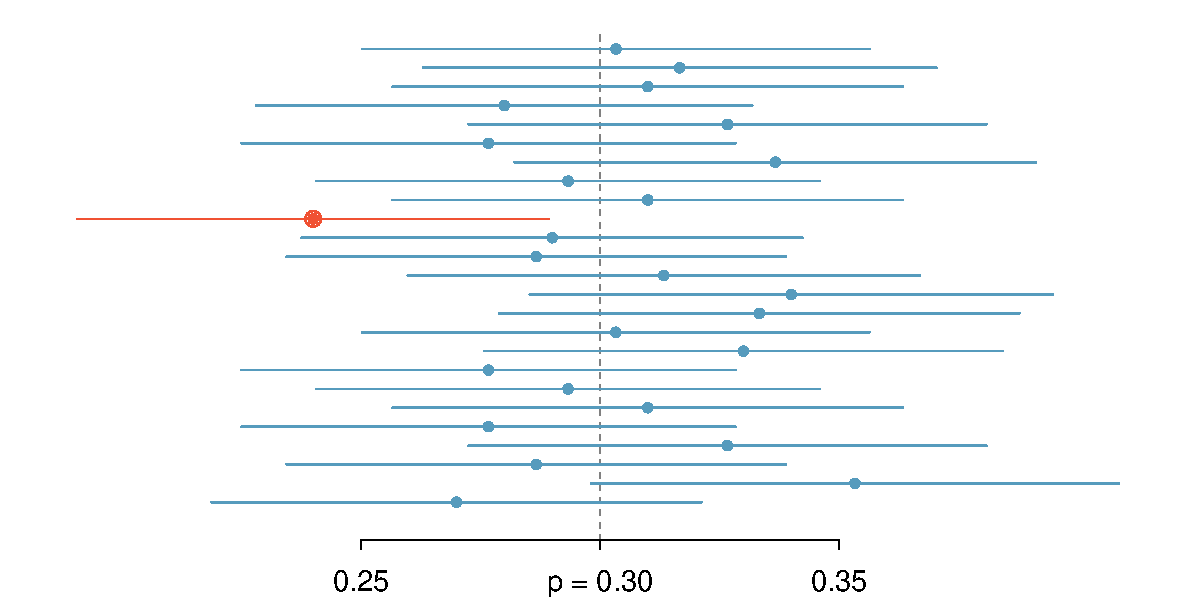
\includegraphics[width=0.95\textwidth]{ch_inference_foundations/figures/95PercentConfidenceInterval/95PercentConfidenceInterval}
\caption{Twenty-five samples of size $n=300$ were simulated when $p = 0.30$. For each sample, a confidence interval was created to try to capture the true proportion $p$. However,~1~of these~25 intervals did not capture $p = 0.30$.}
\label{95PercentConfidenceInterval}
\end{figure}

\textA{\pagebreak}

\begin{exercise}
In Figure~\ref{95PercentConfidenceInterval}, one interval does not contain the true proportion, $p = 0.3$. Does this imply that there was a problem with the simulations?\footnote{No. Just as some observations occur more than 1.96 standard deviations from the mean, some point estimates will be more than 1.96 standard errors from the parameter. A confidence interval only provides a plausible range of values for a parameter. While we might say other values are implausible based on the data, this does not mean they are impossible.}
\end{exercise}


\subsection{Changing the confidence level}
\label{changingTheConfidenceLevelSection}

\index{confidence interval!confidence level|(}

Suppose we want to consider confidence intervals where the confidence level is somewhat higher than 95\%: perhaps we would like a confidence level of 99\%. 

\begin{example}{Would a 99\% confidence interval be wider or narrower than a 95\% confidence interval?}Using a previous analogy: if we want to be more confident that we will catch a fish, we should use a wider net, not a smaller one. To be 99\% confidence of capturing the true value, we must use a wider interval. On the other hand, if we want an interval with lower confidence, such as 90\%, we would use a narrower interval.
\end{example}

The 95\% confidence interval structure provides guidance in how to make intervals with new confidence levels. Below is a general 95\% confidence interval for a point estimate that comes from a nearly normal distribution:
\begin{eqnarray}
\text{point estimate}\ \pm\ 1.96\times SE
\end{eqnarray}
There are three components to this interval: the point estimate, ``1.96'', and the standard error. The choice of $1.96\times SE$ was based on capturing 95\% of the distribution since the estimate is within 1.96 standard deviations of the true value about 95\% of the time. The choice of 1.96 corresponds to a 95\% confidence level. 

\begin{exercise} \label{leadInForMakingA99PercentCIExercise}
If $X$ is a normally distributed random variable, how often will $X$ be within 2.58 standard deviations of the mean?\footnote{This is equivalent to asking how often the Z-score will be larger than -2.58 but less than 2.58. (For a picture, see Figure~\ref{choosingZForCI}.) There is $\approx$ 0.99 probability that the unobserved random variable $X$ will be within 2.58 standard deviations of the mean.}
\end{exercise}

To create a 99\% confidence interval, change 1.96 in the 95\% confidence interval formula to be $2.58$. Guided Practice~\ref{leadInForMakingA99PercentCIExercise} highlights that 99\% of the time a normal random variable will be within 2.58 standard deviations of its mean. This approach -- using the Z-scores in the normal model to compute confidence levels -- is appropriate when the point estimate is associated with a normal distribution and we can properly compute the standard error. Thus, the formula for a 99\% confidence interval is
\begin{eqnarray}
\text{point estimate}\ \pm\ 2.58\times SE
\label{99PercCIForMean}
\label{99PercCIForNormalPointEstimate}
\end{eqnarray}
%\Comment{I don't know where the equation number above gets referenced. Might drop the equation number.}
Figure~\ref{choosingZForCI} provides a picture of how to identify $z^{\star}$ based on a confidence level. 

\begin{figure}[ht]
\centering
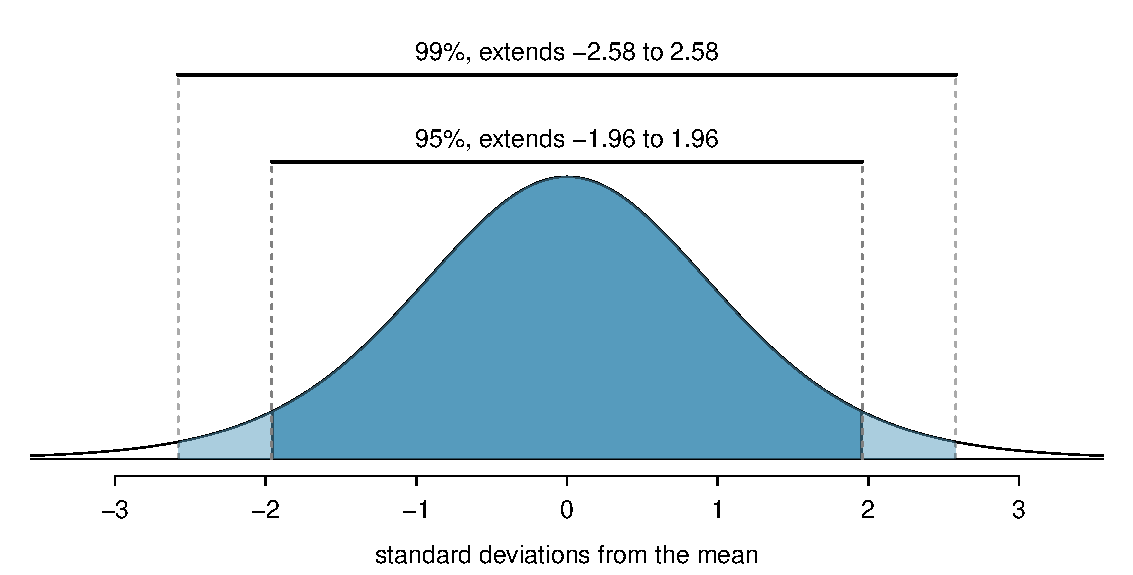
\includegraphics[width=\textwidth]{ch_inference_foundations/figures/choosingZForCI/choosingZForCI}
\caption{The area between -$z^{\star}$ and $z^{\star}$ increases as $|z^{\star}|$ becomes larger. If the confidence level is 99\%, we choose $z^{\star}$ such that 99\% of the normal curve is between -$z^{\star}$ and $z^{\star}$, which corresponds to 0.5\% in the lower tail and 0.5\% in the upper tail: $z^{\star}=2.58$.}
\label{choosingZForCI}
\index{confidence interval!confidence level|)}
\end{figure}

\begin{exercise} \label{find99CIForRun10AgeExercise}
Create a 99\% confidence interval for the impact of the stent on the risk of stroke using the data from Example~\ref{stentStroke95CI_CIsection}. The point estimate is 0.090, and the standard error is $SE = 0.028$. It has been verified for you that the point estimate can reasonably be modeled by a normal distribution.\footnote{Since the necessary conditions for applying the normal model have already been checked for us, we can go straight to the construction of the confidence interval: $\text{point estimate}\ \pm\ 2.58 \times SE \rightarrow (0.018, 0.162)$. We are 99\% confident that implanting a stent in the brain of a patient who is at risk of stroke increases the risk of stroke within 30 days by a rate of 0.018 to 0.162 (assuming the patients are representative of the population).}
\end{exercise}

\begin{termBox}{\tBoxTitle{Confidence interval for any confidence level}
If the point estimate follows the normal model with standard error $SE$, then a confidence interval for the population parameter is
\begin{eqnarray*}
\text{point estimate}\ \pm\ z^{\star} \times SE
\end{eqnarray*}
where $z^{\star}$ depends on the confidence level selected.}
\end{termBox}

Finding the value of $z^{\star}$ that corresponds to a particular confidence level is most easily accomplished by using a new table, called the $t$-table. For now, what is noteworthy about this table is that the bottom row corresponds to confidence levels. The numbers inside the table are the critical values, but which row should we use? Later in this book, we will see that a t curve with infinite degrees of freedom corresponds to the normal curve. For this reason, when finding using the $t$-table to find the appropriate $z^{\star}$, always use row $\infty$.

\begin{table}[hht]
\centering
\begin{tabular}{r | rrr rr}
one tail & \hspace{1.5mm}  0.100 & \hspace{1.5mm} 0.050 & \hspace{1.5mm} 0.025 & \hspace{1.5mm} 0.010 & \hspace{1.5mm} 0.005  \\
\hline
{$df$} \hfill 1  &  {\normalsize  3.078} & {\normalsize  6.314} & {\normalsize 12.71} & {\normalsize 31.82} & {\normalsize 63.66}  \\ 
2  &  {\normalsize  1.886} & {\normalsize  2.920} & {\normalsize  4.303} & {\normalsize  6.965} & {\normalsize  9.925}  \\ 
3  &  {\normalsize  1.638} & {\normalsize  2.353} & {\normalsize  3.182} & {\normalsize  4.541} & {\normalsize  5.841}  \\ 
$\vdots$ & $\vdots$ &$\vdots$ &$\vdots$ &$\vdots$ & \\
1000  &  {\normalsize  1.282} & {\normalsize  1.646} & {\normalsize  1.962} & {\normalsize  2.330} & {\normalsize  2.581}  \\ 
$\infty$   &  {\normalsize  1.282} & {\normalsize  1.645} & {\normalsize  1.960} & {\normalsize  2.326} & {\normalsize  2.576}   \\
\hline
Confidence level C  &  {\normalsize  80\%} & {\normalsize 90\%} & {\normalsize 95\%} & {\normalsize  98\%} & {\normalsize  99\%}  \\
\hline
\end{tabular}
\caption{An abbreviated look at the $t$-table. The columns correspond to confidence levels. Row $\infty$ corresponds to the normal curve.}
\label{tTableSample}
\end{table}


\begin{tipBox}{\tipBoxTitle{Finding $z^{\star}$ for a particular confidence level}
We select $z^{\star}$ so that the area between -$z^{\star}$ and $z^{\star}$ in the normal model corresponds to the confidence level. Use the $t$-table at row $\infty$ to find the critical value $z^{\star}$.}
\end{tipBox}

\begin{exercise} \label{find90CIForRun10AgeExercise}
In Example~\ref{stentStroke95CI_CIsection} we found that implanting a stent in the brain of a patient at risk for a stroke \emph{increased} the risk of a stroke. The study estimated a 9\% increase in the number of patients who had a stroke, and the standard error of this estimate was about $SE = 2.8\%$ or 0.028. Compute a 90\% confidence interval for the effect. Note: the conditions for normality had earlier been confirmed for us.\footnote{We must find $z^{\star}$ such that 90\% of the distribution falls between -$z^{\star}$ and $z^{\star}$ in the standard normal model. Using the $t$-table with a confidence level of 90\% at row $\infty$ gives 1.645. Thus $z^{\star}=1.645$. The 90\% confidence interval can then be computed as
\begin{align*}
\text{point estimate}\ &\pm\ z^{\star}\times SE \\
0.09 \ &\pm \ 1.645\times 0.028 \\
(0.044& \text{ , } 0.136)
\end{align*}
That is, we are 90\% confident that implanting a stent in a stroke patient's brain increased the risk of stroke within 30 days by 4.4\% to 13.6\%.}
\end{exercise}


The normal approximation is crucial to the precision of these confidence intervals. The next two chapters provides detailed discussions about when the normal model can safely be applied to a variety of situations. When the normal model is not a good fit, we will use alternate distributions that better characterize the sampling distribution.

\subsection{Margin of error}

The confidence intervals we have encountered thus far have taken the form
\begin{align*}
\text{point estimate} \ \pm \ z^*\times SE
\end{align*}
Confidence intervals are also often reported as 
\begin{align*}
\text{point estimate} \ \pm \ \text{margin of error}
\end{align*}
For example, instead of reporting an interval as $0.09 \ \pm  \ 1.645\times 0.028$ or $(0.044, 0.136)$, it could be reported as $0.09 \ \pm \  0.046$.

The \term{margin of error} is the distance between the point estimate and the lower or upper bound of a confidence interval.

\begin{termBox}{\tBoxTitle{Margin of error}\label{marginOfErrorTermBox}
A confidence interval can be written as:  point estimate\ $\pm$ \ margin of error.
\newline For a confidence interval for a proportion, the margin of error is $z^{\star}\times SE$.}
\end{termBox}

\begin{exercise}To have a smaller margin or error, should one use a larger sample or a smaller sample?\footnote{Intuitively, a larger sample should tend to yield less error. We can also note that $n$, the sample size is in the denominator of the $SE$ formula, so a $n$ goes up, the $SE$ and thus the margin of error go down.}
\end{exercise}

\begin{exercise}What is the margin of error for the confidence interval: (0.035, 0.145)?\footnote{Because we both add and subtract the margin of error to get the confidence interval, the margin of error is \emph{half} of the width of the interval. $(0.145 - 0.035)/2=0.055$.}
\end{exercise}

\subsection{Interpreting confidence intervals}
\label{interpretingCIs}

\index{confidence interval!interpretation|(}

A careful eye might have observed the somewhat awkward language used to describe confidence intervals. Correct interpretation:
\begin{quote}
We are C\% confident that the true parameter is between \underline{\ \ \ \ \ } and \underline{\ \ \ \ \ }.
\end{quote}
\emph{Incorrect} language might try to describe the confidence interval as capturing the population parameter with a certain probability.\footnote{To see that this interpretation is incorrect, imagine taking two random samples and constructing two 95\% confidence intervals for an unknown proportion. If these intervals are disjoint, can we say that there is a 95\%+95\%=190\% chance that the first or the second interval captures the true value?} This is one of the most common errors: while it might be useful to think of it as a probability, the confidence level only quantifies how plausible it is that the parameter is in the interval.

As we saw in Figure~\ref{95PercentConfidenceInterval}, the 95\% confidence interval \emph{method} has a 95\% probability of producing an interval that will contain the population parameter. A correct interpretation of the confidence \emph{level} is that such intervals will contain the population parameter that percent of the time. However, each individual \emph{interval} either does or does not contain the population parameter. A correct interpretation of an individual confidence interval cannot involve the vocabulary of probability.

Another especially important consideration of confidence intervals is that they \emph{only try to capture the population parameter}. Our intervals say nothing about the confidence of capturing individual observations, a proportion of the observations, or about capturing point estimates. Confidence intervals only attempt to capture population parameters.

\index{confidence interval!interpretation|)}
\index{confidence interval|)}


\subsection{Using confidence intervals: a stepwise approach}

Follow these six steps when carrying out any confidence interval problem. %\Comment{Tweaked term box below, specifically the title, intro, item 3, and item 6.}

%\CommentA{made condition more general}

\begin{termBox}{\tBoxTitle[]{Steps for using confidence intervals (AP exam tip)}
The AP exam is scored in a standardized way, so to ensure full points for a problem, make sure to complete each of the following steps.
\begin{enumerate}
\setlength{\itemsep}{0mm}
\item State the name of the CI being used.
\item Verify conditions to ensure the standard error estimate is reasonable and the point estimate is unbiased and follows the expected distribution, often a normal distribution.
\item Plug in the numbers and write the interval in the form\vspace{-1mm}
\begin{align*}
\text{point estimate}\ \pm\  \text{critical value}\times SE \text{ of estimate}
\end{align*}\vspace{-1mm}% Leave this comment (formatting)
So far, the \term{critical value} has taken the form $z^{\star}$.
\item Evaluate the CI and write in the form (\underline{\ \ \ \ \ }, \underline{\ \ \ \ \ }).
\item Interpret the interval: ``We are C\% confident that the true parameter is between \underline{\ \ \ \ \ } and \underline{\ \ \ \ \ }.  Describe the parameter in context.
\item State your conclusion to the original question. (Sometimes, as in the case of the examples in this section, no conclusion is necessary.)
\end{enumerate}}
\end{termBox}

\index{confidence interval|)}



\textA{\newpage}

\section[Introducing hypothesis testing]{Introducing hypothesis testing \sectionvideohref{youtube-NVbPE1_Cbx8&list=PLkIselvEzpM7Pjo94m1e7J5jkIZkbQAl4} \sectionslideshref{gdoc_aps_slides_5-3}}

\index{hypothesis testing|(}

\begin{example}{Suppose your professor splits the students in class into two groups: students on the left and students on the right. If $\hat{p}_{_L}$ and $\hat{p}_{_R}$ represent the proportion of students who own an Apple product on the left and right, respectively, would you be surprised if $\hat{p}_{_L}$ did not {exactly} equal $\hat{p}_{_R}$?}
While the proportions would probably be close to each other, they are probably not exactly the same. We would probably observe a small difference due to {chance}.
\end{example}

Studying randomness of this form is a key focus of statistics. How large would the observed difference in these two proportions need to be for us to believe that there is a real difference in Apple ownership? In~this section, we'll explore this type of randomness in the context of an unknown proportion, and we'll learn new tools and ideas that will be applied throughout the rest of the book.

\subsection{Case study: medical consultant}

\index{data!medical consultant|(}
People providing an organ for donation sometimes seek the help of a special medical consultant. These consultants assist the patient in all aspects of the surgery, with the goal of reducing the possibility of complications during the medical procedure and recovery. Patients might choose a consultant based in part on the historical complication rate of the consultant's clients.

One consultant tried to attract patients by noting the overall complication rate for liver donor surgeries in the US is about 10\%, but her clients have had only 9 complications in the 142 liver donor surgeries she has facilitated. She claims this is strong evidence that her work meaningfully contributes to reducing complications (and therefore she should be~hired!).

\begin{example}{We will let $p$ represent the true complication rate for liver donors working with this consultant. Estimate $p$ using the data, and label this value $\hat{p}$.}
The sample proportion for the complication rate is 9~complications divided by the 142~surgeries the consultant has worked on: $\hat{p} = 9 / 142 = 0.063$.
\end{example}

\begin{example}{Is it possible to prove that the consultant's work reduces complications?}
No. The claim implies that there is a causal connection, but the data are observational. For example, maybe patients who can afford a medical consultant can afford better medical care, which can also lead to a lower complication rate.
\end{example}

\begin{example}{While it is not possible to assess the causal claim, it is still possible to ask whether the low complication rate of $\hat{p} = 0.063$ provides evidence that the consultant's true complication rate is different than the US complication rate. Why might we be tempted to immediately conclude that the consultant's true complication rate is different than the US complication rate? Can we draw this conclusion?}
Her sample complication rate is $\hat{p} = 0.063$, which is 0.037 lower than the US complication rate of 10\%. However, we cannot yet be sure if the observed difference represents a real difference or is just the result of random variation. We wouldn't expect the sample proportion to be \emph{exactly} 0.10, even if the truth was that her real complication rate was 0.10.
\end{example}


\subsection{Setting up the null and alternate hypothesis}

We can set up two competing hypotheses about the consultant's true complication rate. The first is call the \term{null hypothesis} and represents either a skeptical perspective or a perspective of no difference. The second is called the \term{alternative hypothesis} (or alternate hypothesis) and represents a new perspective such as the possibility that there has been a change or that there is a treatment effect in an experiment.

\begin{termBox}{\tBoxTitle{Null and alternative hypotheses}
\vspace{-5mm}
\begin{description}
\item[] The \term{null hypothesis} is abbreviated $H_0$. It states that nothing has changed and that any deviation from what was expected is due to chance error.
\item[] The \term{alternative hypothesis} is abbreviated $H_A$. It asserts that there has been a change and that the observed deviation is too large to be explained by chance alone.
\end{description}}
\end{termBox}

\begin{example}{Identify the null and alternative claim regarding the consultant's complication rate.}
\begin{itemize}
\item[$H_0$:] The true complication rate for the consultant's clients is the \emph{same as} the US complication rate of~10\%.
\item[$H_A$:] The true complication rate for the consultant's clients is different than~10\%.
\end{itemize}
\end{example}

Often it is convenient to write the null and alternative hypothesis in mathematical or numerical terms. To do so, we must first identify the quantity of interest. This quantity of interest is known as the parameter for a hypothesis test.

\begin{termBox}{\tBoxTitle{Parameters and point estimates}
\vspace{-5mm}
\begin{description}
\item[] A \term{parameter} for a hypothesis test is the ``true'' value of the population of interest. When the parameter is a proportion, we call it $p$.
\item[] A \term{point estimate} is calculated from a sample. When the point estimate is a proportion, we call it $\hat{p}$.
\end{description}
}
\end{termBox}

The observed or sample proportion of 0.063 is a point estimate for the true proportion. The parameter in this problem is the true proportion of complications for this consultant's clients. The parameter is unknown, but the null hypothesis is that it equals the overall proportion of complications: $p = 0.10$. This hypothesized value is called the null value.

\begin{termBox}{\tBoxTitle{Null value of a hypothesis test}
The \term{null value} is the value hypothesized for the parameter in $H_0$, and it is sometimes represented with a~subscript 0, e.g.~$p_0$ (just like $H_0$).}
\end{termBox}

In the medical consultant case study, the parameter is $p$ and the null value is $p_0 = 0.10$. We can write the null and alternative hypothesis as numerical statements as follows.
\begin{itemize}
\item $H_0$: $p=0.10$ (The complication rate for the consultant's clients is equal to the US complication rate of 10\%.)
\item $H_A$: $p \neq 0.10$ (The complication rate for the consultant's clients is not equal to the US complication rate of 10\%.)
\end{itemize}

\begin{termBox}{\tBoxTitle{Hypothesis testing}
These hypotheses are part of what is called a \term{hypothesis test}. A hypothesis test is a statistical technique used to evaluate competing claims using data. Often times, the null hypothesis takes a stance of \emph{no difference} or \emph{no effect}. If the null hypothesis and the data notably disagree, then we will reject the null hypothesis in favor of the alternative hypothesis.\vspace{3mm}

Don't worry if you aren't a master of hypothesis testing at the end of this section. We'll discuss these ideas and details many times in this chapter and the two chapters that follow.}
\end{termBox}

The null claim is always framed as an equality: it tells us what quantity we should use for the parameter when carrying out calculations for the hypothesis test. There are three choices for the alternative hypothesis, depending upon whether the researcher is trying to prove that the value of the parameter is greater than, less than, or not equal to the null value.

\begin{tipBox}{\tipBoxTitle{Always write the null hypothesis as an equality}
We will find it most useful if we always list the null hypothesis as an equality (e.g.~$p = 7$) while the alternative always uses an inequality (e.g. $p \neq 0.7$, $p>0.7$, or~$p<0.7$).}
\end{tipBox}

\begin{exercise}
According to US census data, in 2013 the percent of male residents in the state of Alaska was 52.4\%.\footnote{\oiRedirect{textbook-census_quick_facts_alaska}{quickfacts.census.gov/qfd/states/02000.html}} A researcher plans to take a random sample of residents from Alaska to test whether or not this is still the case. Write out the hypotheses that the researcher should test in both plain and statistical language.~\footnote{$H_0$: $p=0.524$; The proportion of male residents in Alaska is \emph{unchanged} from 2012. $H_A$: $p \neq 0.524$; The proportion of male residents in Alaska has changed from 2012. Note that it could have increased or decreased.}
\end{exercise}

When the alternative claim uses a $\neq$, we call the test a \term{two-sided} test, because either extreme provides evidence against $H_0$. When the alternative claim uses a $<$ or a $>$, we call it a \term{one-sided} test.

\begin{tipBox}{\tipBoxTitle{One-sided and two-sided tests}
If the researchers are only interested in showing an increase or a decrease, but not both, use a one-sided test. If the researchers would be interested in any difference from the null value -- an increase or decrease -- then the test should be two-sided.\vspace{0.5mm}}
\end{tipBox}

\begin{example}{For the example of the consultant's complication rate, we knew that her sample complication rate was 0.063, which was lower than the US complication rate of 0.10. Why did we conduct a two-sided hypothesis test for this setting?}
The setting was framed in the context of the consultant being helpful, but what if the consultant actually performed worse than the US complication rate? Would we care? More than ever! Since we care about a finding in either direction, we should run a two-sided~test.
\end{example}

\begin{caution}{One-sided hypotheses are allowed only \emph{before} seeing data}
{After observing data, it is tempting to turn a two-sided test into a one-sided test. Avoid this temptation. Hypotheses must be set up \emph{before} observing the data. If~they are not, the test must be two-sided.}
\end{caution}

%\begin{termBox}{\tBoxTitle{Point estimates vs parameter}\index{point estimate}\index{parameter}
%Point estimates are calculated based on a sample. For example, the \emph{observed} complication rate for the medical consultant's patients is $\hat{p} = 0.048$. This point estimate is our best guess at the probability $p$ a randomly selected client of hers has a complication. This probability is the parameter and its precise value is never known. However, we can estimate it using the point estimate $\hat{p}$.}
%\end{termBox}

\subsection{Evaluating the hypotheses with a p-value}

\begin{example}
{There were 142 patients in the consultant's sample. If the null claim is true, how many would we expect to have had a complication?}If the null claim is true, we would expect about 10\% of the patients, or about 14.2 to have a complication.
\end{example}

The consultant's complication rate for her 142 clients was 0.063 ($0.063 \times 142 \approx 9$). What is the probability that a sample would produce a number of complications this far from the expected value of 14.2, \emph{if her true complication rate were} 0.10, that~is, if $H_0$ were true? The probability, which is estimated in Section~\ref{MedConsNullNormal} on page~\pageref{MedConsNullNormal}, is about 0.1754. We call this quantity the \term{p-value}.

\begin{figure}[ht]
\centering
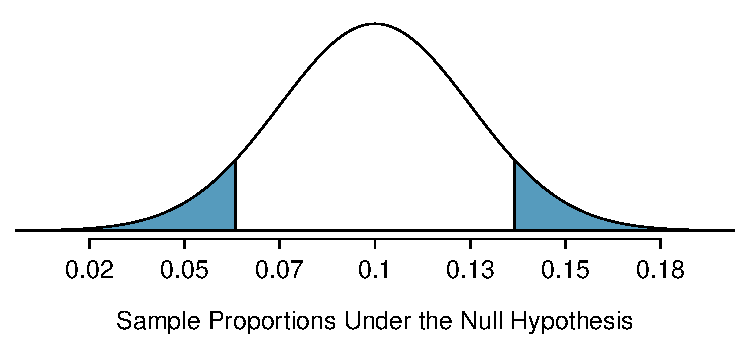
\includegraphics[width=0.7\textwidth]{ch_inference_foundations/figures/MedicalConsultant/MedConsNullNormal}
\caption{The shaded area represents the p-value. We observed $\hat{p} = 0.063$, so any observations smaller than this are at least as extreme relative to the null value, $p_0 = 0.1$, and so the lower tail is shaded. However, since this is a two-sided test, values above 0.137 are also at least as extreme as 0.063 (relative to 0.1), and so they also contribute to the p-value. The tail areas together total of about 0.1754 when calculated using a simulation technique in Section~\ref{calcPValueUsingSimulationSubSection}.}
\label{MedConsNullNormal}
\end{figure}

\begin{figure}[ht]
\centering
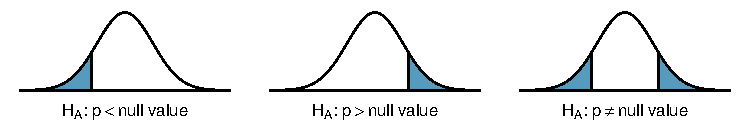
\includegraphics[width=\textwidth]{ch_inference_foundations/figures/sidedness/sidedness_example_figures}
\caption{When the alternative hypothesis takes the form $p <$ null value, the p-value is represented by the lower tail. When it takes the form $p >$ null value, the p-value is represented by the upper tail. When using $p \neq$ null value, then the p-value is represented by both tails.}
\label{sidedness_example_figures}
\end{figure}

\textA{\newpage}

\begin{termBox}{\tBoxTitle{Finding and interpreting the p-value}
When examining a proportion, we find and interpret the \term{p-value}\index{hypothesis testing!p-value|textbf} according to the nature of the alternative hypothesis.\vspace{-1mm}
\begin{description}
\setlength{\itemsep}{0mm}
\item[$H_A$: $p > p_0.$ ] The p-value is the probability of observing a sample proportion as large as we saw in our sample, if the null hypothesis were true. The p-value corresponds to the area in the \emph{upper} tail.
\item[$H_A$: $p < p_0.$ ]The p-value is the probability of observing a sample proportion as small as we saw in our sample, if the null hypothesis were true. The p-value corresponds to the area in the \emph{lower} tail.
\item[$H_A$: $p \ne p_0.$] The p-value is the probability of observing a sample proportion as far from the null value as what was observed in the current data set, if the null hypothesis were true. The p-value corresponds to the area in \emph{both} tails.
\end{description}}
\end{termBox}

When the p-value is small, i.e. less than a previously set threshold, we say the results are \term{statistically significant}. This means the data provide such strong evidence against $H_0$ that we reject the null hypothesis in favor of the alternative hypothesis. The threshold, called the \term{significance level}\index{hypothesis testing!significance level}\index{significance level} and often represented by $\alpha$ (the Greek letter \emph{alpha}\label{alphadiscussion})\marginpar[\raggedright\vspace{-4mm}

$\alpha$\\\footnotesize significance\\level of a\\hypothesis test]{\raggedright\vspace{-4mm}

$\alpha$\\\footnotesize significance\\level of a\\hypothesis test}, is typically set to $\alpha = 0.05$, but can vary depending on the field or the application. %Using a significance level of $\alpha = 0.05$ in the discrimination study, we can say that the data did not provide statistically significant evidence against the null hypothesis, because the p-value of 0.1754 was larger than the $\alpha$ of 0.05.

\begin{termBox}{\tBoxTitle{Statistical significance}
If the p-value is less than the significance level $\alpha$ (usually 0.05), we say that the result is \term{statistically significant}\index{hypothesis testing!statistically significant|textbf}. We reject $H_0$, and we have strong evidence favoring~$H_A$. \\[2mm]
If the p-value is greater than the significance level $\alpha$, we say that the result is not statistically significant. We do not reject $H_0$, and we do not have strong evidence for $H_A$.}
\end{termBox}

Recall that the null claim is the claim of no difference. If we reject $H_0$, we are asserting that there is a real difference. If we do not reject $H_0$, we are saying that the null claim is reasonable, but \emph{it has not been proven}.

\begin{exercise} \label{plainLanguageExplanationOfHTConclusionForLiverDonorSurgicalConsultant}
Because the p-value is 0.1754, which is larger than the significance level 0.05, we do not reject the null hypothesis. Explain what this means in the context of the problem using plain language.\footnote{The data do not provide evidence that the consultant's complication rate is significantly lower or higher that the US complication rate of 10\%.}
\end{exercise}

\begin{example}{In the previous exercise, we did not reject $H_0$. This means that we did not disprove the null claim. Is this equivalent to proving the null claim is~true?}
No. We did not prove that the consultant's complication rate is \emph{exactly} equal to 10\%. Recall that the test of hypothesis starts by \emph{assuming the null claim is true}. That~is, the test proceeds as an argument by contradiction. \emph{If the null claim is true}, there is a 0.1754 chance of seeing sample data as divergent from 10\% as we saw in our sample. Because 0.1754 is large, it is within the realm of chance error and we cannot say the null hypothesis is unreasonable.\footnote{The p-value is actually a conditional probability. It is P(getting data at least as divergent from the null value as we observed $|$ $H_0$ is true). It is NOT P( $H_0$ is true $|$ we got data this divergent from the null value.}
\end{example}


\begin{tipBox}{\tipBoxTitle{Double negatives can sometimes be used in statistics}
In many statistical explanations, we use double negatives. For instance, we might say that the null hypothesis is \emph{not implausible} or we \emph{failed to reject} the null hypothesis. Double negatives are used to communicate that while we are not rejecting a position, we are also not saying that we know it to be true.}
\end{tipBox}

\begin{example}{Does the conclusion in Guided Practice~\ref{plainLanguageExplanationOfHTConclusionForLiverDonorSurgicalConsultant} ensure that there is no real association between the surgical consultant's work and the risk of complications? Explain.}
No. It is possible that the consultant's work is associated with a lower or higher risk of complications. However, the data did not provide enough information to reject the null hypothesis (the sample was too small).
\index{data!medical consultant|)}
\end{example}

%The 2-in-100 chance is what we call a \term{p-value}, which is a probability quantifying the strength of the evidence against the null hypothesis and in favor of the alternative. %Formally the p-value is a conditional probability, which is basically\footnote{Want to learn more probability? Check out~Appendix~\ref{probability}.}


%\begin{termBox}{\tBoxTitle{Significance level}
%If the null hypothesis is true, the significance level $\alpha$ defines the probability that we will make a Type~1 Error.}
%\end{termBox}

\begin{example}{An experiment was conducted where study participants were randomly divided into two groups. Both were given the opportunity to purchase a DVD, but the one half was reminded that the money, if not spent on the DVD, could be used for other purchases in the future while the other half was not. The half that were reminded that the money could be used on other purchases were 20\% less likely to continue with a DVD purchase. We determined that such a large difference would only occur about 1-in-150 times if the reminder actually had no influence on student decision-making. What is the p-value in this study? Was the result statistically significant?}
The p-value was 0.006 (about 1/150). Since the p-value is less than 0.05, the data provide statistically significant evidence that US college students were actually influenced by the reminder.
\end{example}

\begin{termBox}{\tBoxTitle{What's so special about 0.05?}
We often use a threshold of 0.05 to determine whether a result is statistically significant. But why 0.05? Maybe we should use a bigger number, or maybe a smaller number. If you're a little puzzled, that probably means you're reading with a critical eye -- good job! We've made a video to help clarify \emph{why 0.05}:
\begin{center}
\oiRedirect{textbook-why05}{www.openintro.org/why05}
\end{center}
Sometimes it's also a good idea to deviate from the standard. We'll discuss when to choose a threshold different than 0.05 in Section~\ref{significanceLevel}.\vspace{0.5mm}}
\end{termBox}

Statistical inference is the practice of making decisions and conclusions from data in the context of uncertainty. Just as a confidence interval may occasionally fail to capture the true parameter, a test of hypothesis may occasionally lead us to an incorrect conclusion. While a given data set may not always lead us to a correct conclusion, statistical inference gives us tools to control and evaluate how often these errors occur.


\subsection{Calculating the p-value by simulation (special topic)}
\label{calcPValueUsingSimulationSubSection}

When conditions for the applying the normal model are met, we use the normal model to find the p-value of a test of hypothesis. In the complication rate example, the distribution is not normal. It is, however, \emph{binomial}, because we are interested in how many out of 142 patients will have complications.

We could calculate the p-value of this test using binomial probabilities. A more general approach, though, for calculating p-values when the normal model does not apply is to use what is known as \term{simulation}. While performing this procedure is outside of the scope of the course, we provide an example here in order to better understand the concept of a p-value.

We simulate 142 new patients to see what result might happen if the complication rate really is 0.10. To do this, we could use a deck of cards. Take one red card, nine black cards, and mix them up. If the cards are well-shuffled, drawing the top card is one way of simulating the chance a patient has a complication if the true rate is 0.10: if the card is red, we say the patient had a complication, and if it is black then we say they did not have a complication. If we repeat this process 142 times and compute the proportion of simulated patients with complications, $\hat{p}_{sim}$, then this simulated proportion is exactly a draw from the null distribution.

There were 12 simulated cases with a complication and 130 simulated cases without a complication: $\hat{p}_{sim} = 12 / 142 = 0.085$.

One simulation isn't enough to get a sense of the null distribution, so we repeated the simulation 10,000 times using a~computer. Figure~\ref{MedConsNullSim} shows the null distribution from these 10,000 simulations. The simulated proportions that are less than or equal to $\hat{p}=0.063$ are shaded. There were 0.0877 simulated sample proportions with $\hat{p}_{sim} \leq 0.063$, which represents a fraction 0.0877 of our simulations:
\begin{align*}
\text{left tail }
	= \frac{\text{Number of observed simulations with }\hat{p}_{sim}\leq\text{ 0.063}}{10000}
	= \frac{877}{10000} = 0.0877
\end{align*}
However, this is not our p-value! Remember that we are conducting a two-sided test, so we should double the one-tail area to get the p-value:\footnote{This doubling approach is preferred even when the distribution isn't symmetric, as in this case.}
\begin{align*}
\text{p-value} = 2 \times \text{left tail} = 2 \times 0.0877 = 0.1754
\end{align*}

\begin{figure}[ht]
\centering
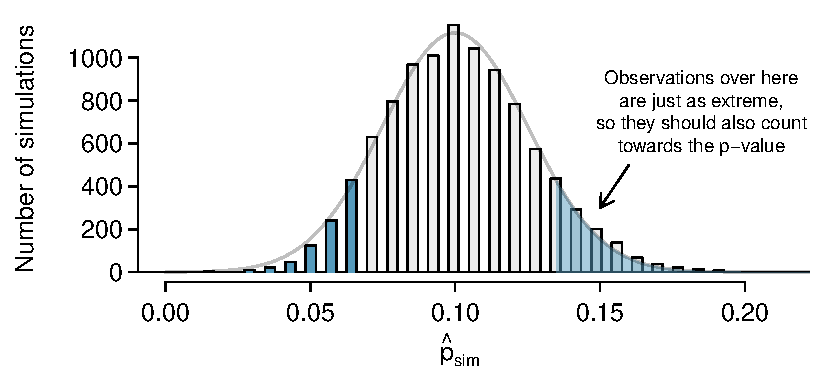
\includegraphics[width=0.8\textwidth]{ch_inference_foundations/figures/MedicalConsultant/MedConsNullSim}
\caption{The null distribution for $\hat{p}$, created from 10,000 simulated studies. The left tail contains 8.77\% of the simulations. For a two-sided test, we double the tail area to get the p-value. This doubling accounts for the observations we might have observed in the upper tail, which are also at least as extreme (relative to 0.10) as what we observed, $\hat{p} = 0.063$.}
\label{MedConsNullSim}
\end{figure}

\subsection{Formal hypothesis testing: a stepwise approach}

\begin{termBox}{\tBoxTitle{Carrying out a formal test of hypothesis (AP exam tip)}
Follow these seven steps when carrying out a hypothesis test. 
\begin{enumerate}
\setlength{\itemsep}{0mm}
\item State the name of the test being used.
\item Verify conditions to ensure the standard error estimate is reasonable and the point estimate follows the appropriate distribution and is unbiased.
\item Write the hypotheses in plain language, then set them up in mathematical notation.
\item Identify the significance level $\alpha$.
\item Calculate the test statistic, often Z, using an appropriate point estimate of the parameter of interest and its standard error.\vspace{-1.5mm}
\begin{align*}
\text{test statistic} = \frac{\text{point estimate} - \text{null value}}{SE \text{ of estimate}}
\end{align*}
\item Find the p-value, compare it to $\alpha$, and state whether to reject or not reject the null hypothesis.
\item Write your conclusion in context.
\end{enumerate}}
\end{termBox}

\subsection{Decision errors}
\index{hypothesis testing!decision errors|(}
The hypothesis testing framework is a very general tool, and we often use it without a second thought. If a person makes a somewhat unbelievable claim, we are initially skeptical. However, if there is sufficient evidence that supports the claim, we set aside our skepticism. The hallmarks of hypothesis testing are also found in the US court system. 

\begin{example}{A US court considers two possible claims about a defendant: she is either innocent or guilty. If we set these claims up in a hypothesis framework, which would be the null hypothesis and which the alternative?}\label{hypTestCourtExample}
The jury considers whether the evidence is so convincing (strong) that there is no reasonable doubt of the person's guilt. That is, the skeptical perspective (null hypothesis) is that the person is innocent until evidence is presented that convinces the jury that the person is guilty (alternative hypothesis). In statistics, our evidence comes in the form of data, and we use the significance level to decide what is beyond a reasonable doubt.
\end{example}

Jurors examine the evidence to see whether it convincingly shows a defendant is guilty. Notice that a jury finds a defendent either guilty or not guilty. They either reject the null claim or they do not reject the null claim. They never prove the null claim, that is, they never find the defendant innocent. If a jury finds a defendant \emph{not guilty}, this does not necessarily mean the jury is confident in the person's innocence. They are simply not convinced of the alternative that the person is guilty.

This is also the case with hypothesis testing: \emph{even if we fail to reject the null hypothesis, we typically do not accept the null hypothesis as truth}. Failing to find strong evidence for the alternative hypothesis is not equivalent to providing evidence that the null hypothesis is true.


Hypothesis tests are not flawless. Just think of the court system: innocent people are sometimes wrongly convicted and the guilty sometimes walk free. Similarly, data can point to the wrong conclusion. However, what distinguishes statistical hypothesis tests from a court system is that our framework allows us to quantify and control how often the data lead us to the incorrect conclusion.

There are two competing hypotheses: the null and the alternative. In a hypothesis test, we make a statement about which one might be true, but we might choose incorrectly. There are four possible scenarios in a hypothesis test, which are summarized in Table~\ref{fourHTScenarios}.

\begin{table}[ht]
\centering
\begin{tabular}{l l c c c}
& & \multicolumn{2}{c}{\textbf{Test conclusion}} \\
  \cline{3-4}
\vspace{-3.7mm} \\
& & do not reject $H_0$ &  reject $H_0$ in favor of $H_A$ &
\ \hspace{7mm} \  \\
  \cline{2-4}
\vspace{-3.7mm} \\
& $H_0$ true & okay &  Type~1 Error \\
\raisebox{1.5ex}{\textbf{Truth}} & $H_A$ true & Type~2 Error & okay \\
  \cline{2-4}
\end{tabular}
\caption{Four different scenarios for hypothesis tests.}
\label{fourHTScenarios}
\end{table}

\begin{termBox}{\tBoxTitle{Type~1 and Type~2 Errors}
A \term{Type~1 Error} is rejecting the null hypothesis when $H_0$ is actually true. When we reject the null hypothesis, it is possible that we make a Type~1 Error. \\[2mm]
A \term{Type~2 Error} is failing to reject the null hypothesis when $H_A$ is actually true.}
\end{termBox}



\begin{example}{In a US court, the defendant is either innocent ($H_0$) or guilty ($H_A$). What does a Type~1 Error represent in this context? What does a Type~2 Error represent? Table~\ref{fourHTScenarios} may be useful.}
If the court makes a Type~1 Error, this means the defendant is innocent ($H_0$ true) but wrongly convicted. A~Type~2 Error means the court failed to reject $H_0$ (i.e. failed to convict the person) when she was in fact guilty ($H_A$ true).
\end{example}

\begin{example}{How could we reduce the Type~1 Error rate in US courts? What influence would this have on the Type~2 Error rate?}
To lower the Type~1 Error rate, we might raise our standard for conviction from ``beyond a reasonable doubt'' to ``beyond a conceivable doubt'' so fewer people would be wrongly convicted. However, this would also make it more difficult to convict the people who are actually guilty, so we would make more Type~2 Errors.
\end{example}

\begin{exercise} \label{howToReduceType2ErrorsInUSCourts}
How could we reduce the Type~2 Error rate in US courts? What influence would this have on the Type~1 Error rate?\footnote{To lower the Type~2 Error rate, we want to convict more guilty people. We could lower the standards for conviction from ``beyond a reasonable doubt'' to ``beyond a little doubt''. Lowering the bar for guilt will also result in more wrongful convictions, raising the Type~1 Error rate.}
\end{exercise}

\begin{exercise}
A group of women bring a class action lawsuit that claims discrimination in promotion rates. What would a Type~1 Error represent in this context?\footnote{We must first identify which is the null hypothesis and which is the alternative. The alternative hypothesis is the one that bears the burden of proof, so the null hypothesis is that there was no discrimination and the alternative hypothesis is that there was discrimination. Making a Type~1 Error in this context would mean that in fact there was no discrimination, even though we concluded that women were discriminated against. Notice that this does \emph{not} necessarily mean something was wrong with the data or that we made a computational mistake. Sometimes data simply point us to the wrong conclusion, which is why scientific studies are often repeated to check initial findings.}
\end{exercise}

\index{hypothesis testing!decision errors|)}

The example and Exercise above provide an important lesson: if we reduce how often we make one type of error, we generally make more of the other type.

%Hypothesis testing is built around rejecting or failing to reject the null hypothesis. That is, we do not reject $H_0$ unless the data provide strong evidence against it. But what precisely does \emph{strong evidence} mean? As a general rule of thumb, for those cases where the null hypothesis is actually true, we do not want to incorrectly reject $H_0$ more than 5\% of the time. This corresponds to our default significance level of $\alpha = 0.05$, which we use as a comparison with the p-value. In the next section, we discuss the appropriateness of different significance levels.


\subsection{Choosing a significance level}
\label{significanceLevel}

\index{hypothesis testing!significance level|(}
\index{significance level|(}

If $H_0$ is true, what is the probability that we will incorrectly reject it? In hypothesis testing, we perform calculations under the premise that $H_0$ is true, and we reject $H_0$ if the p-value is smaller than the significance level $\alpha$. That is, $\alpha$ \emph{is} the probability of making a Type~1 Error. The choice of what to make $\alpha$ is not arbitrary. It depends on the gravity of the consequences of a Type~1 Error.

\begin{termBox}{\tBoxTitle{Relationship between Type~1 and Type~2 Errors}
The probability of a Type~1 Error is called $\alpha$ and corresponds to the significance level of a test. The probability of a Type~2 Error is called $\beta$. As we make $\alpha$ smaller, $\beta$ typically gets larger, and vice versa.}
\end{termBox}

\begin{example}{If making a Type~1 Error is especially dangerous or especially costly, should we choose a smaller significance level or a higher significance level?}
Under this scenario, we want to be very cautious about rejecting the null hypothesis, so we demand very strong evidence before we are willing to reject the null hypothesis. Therefore, we want a smaller significance level, maybe $\alpha = 0.01$.
\end{example}

\begin{example}{If making a Type~2 Error is especially dangerous or especially costly, should we choose a smaller significance level or a higher significance level?}
We should choose a higher significance level (e.g. 0.10). Here we want to be cautious about failing to reject $H_0$ when the null is actually false.
\end{example}

\begin{tipBox}{\tipBoxTitle{Significance levels should reflect consequences of errors}
The significance level selected for a test should reflect the real-world consequences associated with making a Type~1 or Type~2 Error. If a Type~1 Error is very dangerous, make $\alpha$ smaller.}
\end{tipBox}

\index{hypothesis testing!significance level|)}
\index{significance level|)}


\subsection{Statistical power of a hypothesis test}

When the alternative hypothesis is true, the probability of \underline{not} making a Type~2 Error is called \term{power}. It is common for researchers to perform a \hiddenterm{power analysis} to ensure their study collects enough data to detect the effects they anticipate finding. As you might imagine, if the effect they care about is small or subtle, then if the effect is real, the researchers will need to collect a large sample size in order to have a good chance of detecting the effect. However, if they are interested in large effect, they need not collect as much data.

The Type~2 Error rate $\beta$ and the magnitude of the error for a point estimate are controlled by the sample size. As the sample size $n$ goes up, the Type~2 Error rate goes down, and power goes up. Real differences from the null value, even large ones, may be difficult to detect with small samples. However, if we take a very large sample, we might find a statistically significant difference but the magnitude might be so small that it is of no practical value.

\index{hypothesis testing|)}



%__________________
\section{Does it make sense?}
\subsection{When to retreat}
\label{whenToRetreat}

Statistical tools rely on conditions. When the conditions are not met, these tools are unreliable and drawing conclusions from them is treacherous. The conditions for these tools typically come in two forms.
\begin{itemize}
\setlength{\itemsep}{0mm}
\item \textbf{The individual observations must be independent.} A random sample from less than 10\% of the population ensures the observations are independent. In experiments, we generally require that subjects are randomized into groups. If independence fails, then advanced techniques must be used, and in some such cases, inference may not be possible.
\item \textbf{Other conditions focus on sample size and skew.} For example, if the sample size is too small, the skew too strong, or extreme outliers are present, then the normal model for the sample mean will fail.
\end{itemize}
Verification of conditions for statistical tools is always necessary. Whenever conditions are not satisfied for a statistical technique, there are three options. The first is to learn new methods that are appropriate for the data. The second route is to consult a statistician.\footnote{If you work at a university, then there may be campus consulting services to assist you. Alternatively, there are many private consulting firms that are also available for hire.} The third route is to ignore the failure of conditions. This last option effectively invalidates any analysis and may discredit novel and interesting findings.

Finally, we caution that there may be no inference tools helpful when considering data that include unknown biases, such as convenience samples. For this reason, there are books, courses, and researchers devoted to the techniques of sampling and experimental design. See Sections~\ref{overviewOfDataCollectionPrinciples}-\ref{experimentsSection} for basic principles of data collection.


\textA{\newpage}

\subsection{Statistical significance versus practical significance}

When the sample size becomes larger, point estimates become more precise and any real differences in the mean and null value become easier to detect and recognize. Even a very small difference would likely be detected if we took a large enough sample. Sometimes researchers will take such large samples that even the slightest difference is detected. While we still say that difference is \term{statistically significant}, it might not be \term{practically significant}.

Statistically significant differences are sometimes so minor that they are not practically relevant. This is especially important to research: if we conduct a study, we want to focus on finding a meaningful result. We don't want to spend lots of money finding results that hold no practical value.

The role of a statistician in conducting a study often includes planning the size of the study. The statistician might first consult experts or scientific literature to learn what would be the smallest meaningful difference from the null value. She also would obtain some reasonable estimate for the standard deviation. With these important pieces of information, she would choose a sufficiently large sample size so that the power for the meaningful difference is perhaps 80\% or 90\%. While larger sample sizes may still be used, she might advise against using them in some cases, especially in sensitive areas of research.

